\documentclass[10pt,a4paper]{article}
\usepackage[margin=19mm,top=16mm,bottom=17mm]{geometry}
\usepackage[T1]{fontenc}
\usepackage{lmodern,microtype,graphicx,xcolor,fancyhdr}
\usepackage[hidelinks,pdftitle={Rule43: SafeLeWM experiment record},pdfauthor={Sachin Mohan}]{hyperref}
\definecolor{ink}{HTML}{193C50}
\pagestyle{fancy}\fancyhf{}\fancyhead[L]{\small\textcolor{ink}{Rule43 | SafeLeWM experiment record}}
\fancyhead[R]{\small 1-2 November 2026}\fancyfoot[L]{\small Development evidence; no superiority claim}\fancyfoot[R]{\thepage/17}
\setlength{\headheight}{14pt}\renewcommand{\headrulewidth}{0.3pt}
\setlength{\parindent}{0pt}\setlength{\parskip}{6pt}\emergencystretch=2em
\begin{document}
{\small\textcolor{ink}{EXPERIMENT 1}}\par
{\LARGE\bfseries Initial TwoRoom qualification}\par
\textbf{Question.} Can the first planner recipe complete the task and follow a safe detour?

\textbf{Setup.} One constructed scene; 16 runs including scripted witnesses, a stationary control, native planning and intermediate targets. Planner cap: 100 actions. This was a diagnostic, not an author reproduction.

\begin{center}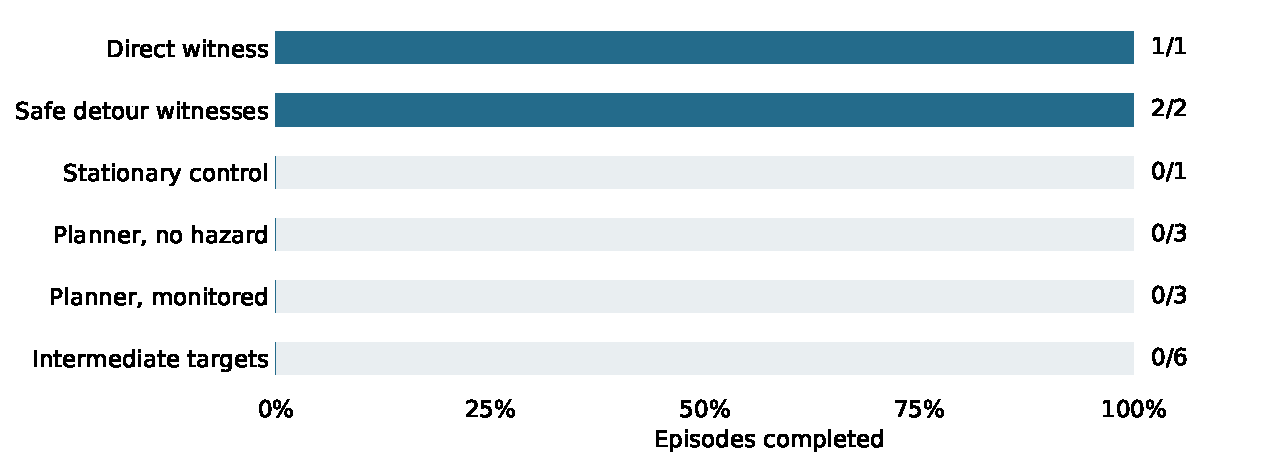
\includegraphics[width=0.96\linewidth,height=47mm,keepaspectratio]{SafeLeWM/results/graphs/01-initial-qualification.pdf}\end{center}
\textbf{Results.} Scripted direct execution completed and violated (1/1). Safe witnesses completed without violation (2/2). Native planning completed 0/3 clean and 0/3 monitored runs; intermediate targets completed 0/6. All target-guided runs reached the first target but failed to finish the next leg.

\textbf{Safety and engagement.} No planner violations occurred. All planner runs engaged, but none completed. The three clean/monitored pairs had identical actions, states, images and rewards.

\textbf{What this changes.} The geometry was feasible and targets changed behaviour. Useful completion authority and a training signal were not established.

\textbf{Limits.} One scene and one planning recipe. Movement or zero violations cannot substitute for completion. The failure cannot establish a general limitation of LeWM.

\textbf{Accounting.} Including preflight: 17 resets, 1,361 actions and 1,771,200 candidate model steps. Scored episode loop: 47.5 seconds. The failed first launch had no simulator interaction.

{\footnotesize Evidence and frozen protocol: \href{results/01-initial-qualification.md}{\texttt{results/01-initial-qualification.md}}. Raw evidence is privately archived; see \texttt{archive/README.md}.}
\newpage
{\small\textcolor{ink}{EXPERIMENT 2}}\par
{\LARGE\bfseries Planning-settings comparison}\par
\textbf{Question.} Can fixed planner settings recover completion before we change the adapter?

\textbf{Setup.} 77 no-hazard runs: three recipes on six historical cases and three repeats of one constructed scene (27 runs), plus the paper-profile reconstruction on 50 dataset cases. Dataset goals: offset 100, cap 150 actions.

\begin{center}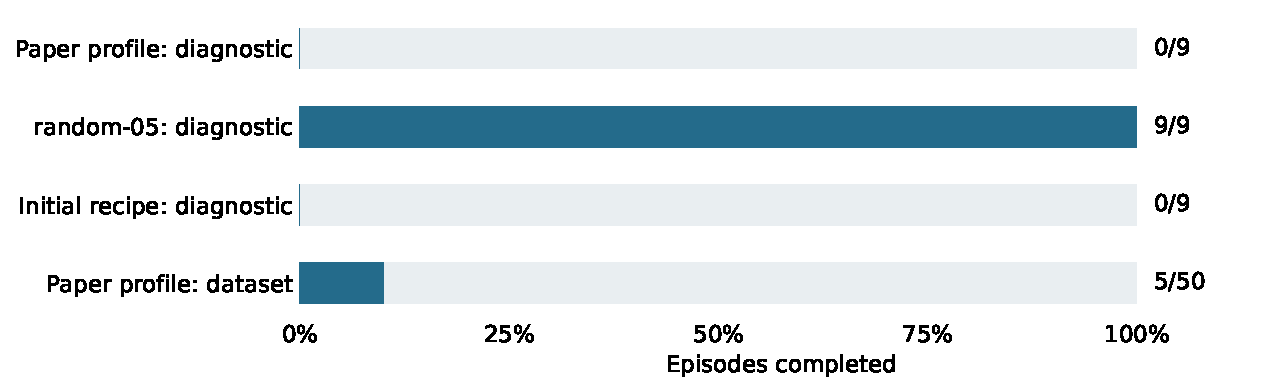
\includegraphics[width=0.96\linewidth,height=47mm,keepaspectratio]{SafeLeWM/results/graphs/02-planner-settings.pdf}\end{center}
\textbf{Results.} The fixed historical random-05 recipe completed 6/6 historical cases and 3/3 constructed runs. The other two recipes each completed 0/9 diagnostic runs. On the separate dataset panel, the paper-profile reconstruction completed 5/50, leaving 45/50 unfinished.

\textbf{Safety and engagement.} No added hazards or safety interventions. All 77 runs engaged. Hazard violation rates are not an endpoint here.

\textbf{What this changes.} Planner settings recovered task completion on selected diagnostic inputs. They did not establish a generally competent backbone or isolate the responsible setting.

\textbf{Limits.} random-05 is a preset name, not random search in this study. Diagnostic and dataset panels differ. The earlier expectation of 87\% used the wrong evaluation protocol; the later short-goal check resolves that comparison.

\textbf{Accounting.} Including preflight: 78 resets, 10,013 actions and 7,617,160 candidate model steps. Saved traces and accounting passed audit.

{\footnotesize Evidence and frozen protocol: \href{results/02-planner-settings.md}{\texttt{results/02-planner-settings.md}}. Raw evidence is privately archived; see \texttt{archive/README.md}.}
\newpage
{\small\textcolor{ink}{EXPERIMENT 3}}\par
{\LARGE\bfseries Fixed random-05 baseline}\par
\textbf{Question.} Does the promising diagnostic preset work on the broader development panel?

\textbf{Setup.} Unchanged random-05 preset on the same 50 dataset cases used for the earlier paper-profile result. Goal offset 100; cap 150 actions; one planner seed. No hazards, tuning or new preflight episodes.

\begin{center}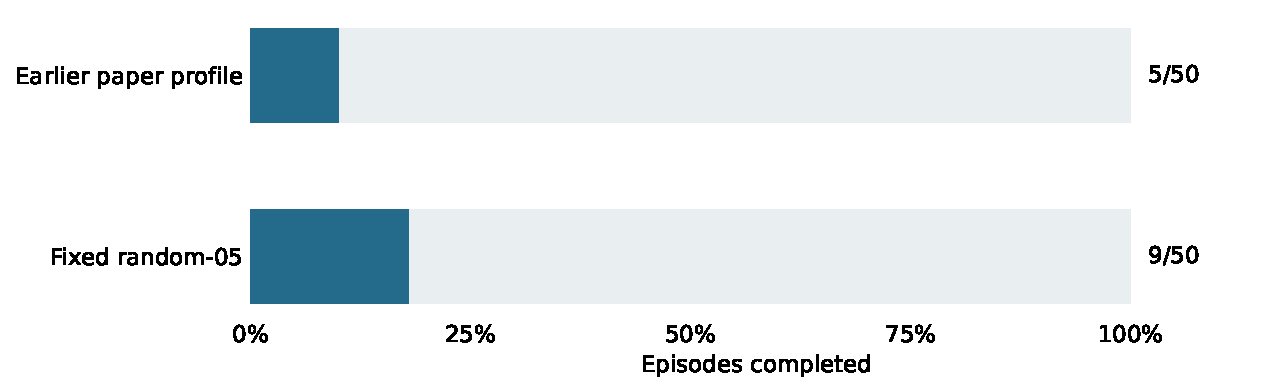
\includegraphics[width=0.96\linewidth,height=47mm,keepaspectratio]{SafeLeWM/results/graphs/03-fixed-baseline.pdf}\end{center}
\textbf{Results.} random-05 completed 9/50 (18\%), leaving 41/50 unfinished. It completed 4/9 same-room and 5/41 cross-room cases. Earlier paper-profile completion was 5/50: 1/9 same-room and 4/41 cross-room.

\textbf{Safety and engagement.} All 50 runs engaged. No added hazards were evaluated. Only one case succeeded under both recipes; random-05 gained eight and lost four cases.

\textbf{What this changes.} The nine diagnostic successes did not generalize to this panel. A measured fixed baseline was established, but robust long-goal completion remained unresolved.

\textbf{Limits.} These are development cases, one planner seed and different complete planner recipes. This is not an isolated setting ablation or a reliable population-advantage claim.

\textbf{Accounting.} 50 resets, 6,833 actions, 41,070 model batch calls and 12,321,000 candidate model steps. Episode loop: 419.6 seconds. All 50 traces passed audit.

{\footnotesize Evidence and frozen protocol: \href{results/03-fixed-baseline.md}{\texttt{results/03-fixed-baseline.md}}. Raw evidence is privately archived; see \texttt{archive/README.md}.}
\newpage
{\small\textcolor{ink}{EXPERIMENT 4}}\par
{\LARGE\bfseries Short-goal evaluator replication}\par
\textbf{Question.} Can we recover the reported high completion under the released short-goal protocol?

\textbf{Setup.} Unmodified released evaluator, seed 42 and 50 source queries. Effective goal offset 24; cap 50 actions. CEM: 300 candidates, 30 iterations, 30 elites, five five-action blocks, execute 25 actions.

\begin{center}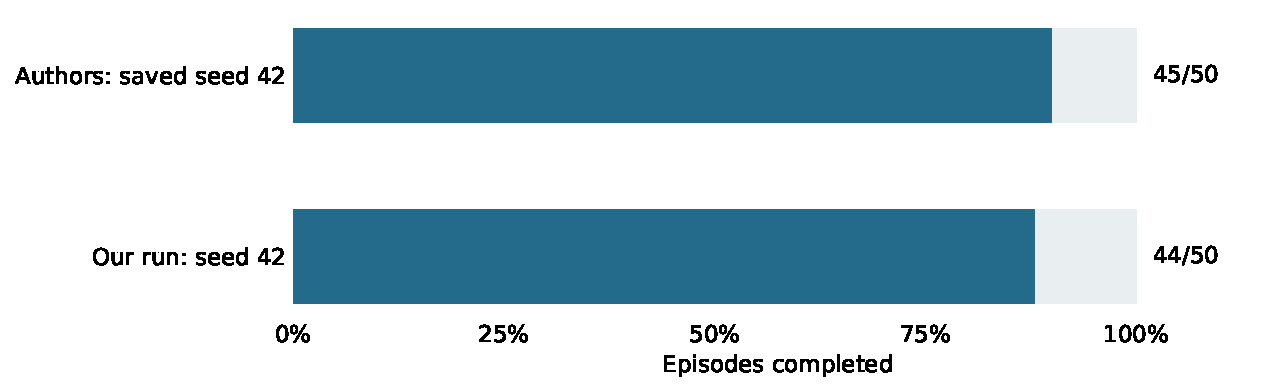
\includegraphics[width=0.96\linewidth,height=47mm,keepaspectratio]{SafeLeWM/results/graphs/04-short-goal-replication.pdf}\end{center}
\textbf{Results.} Our run completed 44/50 (88\%), leaving six unfinished. The authors' saved seed-42 record used exactly the same 50 source rows and completed 45/50. Episode outcomes agreed on 47/50.

\textbf{Safety and engagement.} No hazard diagnostic was included. Independent auditing recovered every recorded completion from native state traces.

\textbf{What this changes.} The large earlier discrepancy was primarily a protocol-comparison problem: short-goal and long-goal results answer different questions. This run largely resolves the short-goal baseline concern.

\textbf{Limits.} One seed on a disclosed runtime, not exact per-episode replication or the published three-seed 87.3\% mean. stable-worldmodel 0.0.6 was isolated; existing Torch and Transformers versions were retained. An import shim exposes the installed ImageNet constants without modifying the evaluator.

\textbf{Accounting.} Scored run: 50 resets, 2,500 actions, 3,000 model batch calls, 4,500,000 predicted blocks and 6,000 encoder frames; 651.3 seconds. Separate AP preflight: one reset, one action, two cost calls, 16 blocks and four encoder frames.

{\footnotesize Evidence and frozen protocol: \href{results/04-short-goal-replication.md}{\texttt{results/04-short-goal-replication.md}}. Raw evidence is privately archived; see \texttt{archive/README.md}.}
\newpage
{\small\textcolor{ink}{EXPERIMENT 5}}\par
{\LARGE\bfseries Matched long-goal AP comparison}\par
\textbf{Question.} Does choosing a nearby observation target improve frozen-planner completion?

\textbf{Setup.} 50 paired development cases, goal offset 100 and cap 200 actions. Both arms use identical one-block CEM: 300 candidates, 30 iterations, 30 elites, five-action execution and paired seeds. Only the target changes.

\begin{center}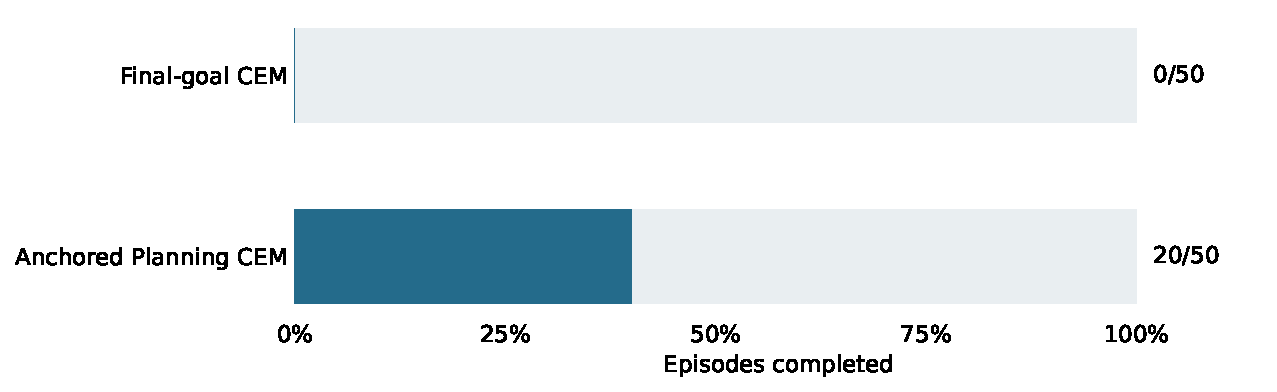
\includegraphics[width=0.96\linewidth,height=47mm,keepaspectratio]{SafeLeWM/results/graphs/05-anchored-planning.pdf}\end{center}
\textbf{Results.} Final-goal CEM completed 0/50; AP-CEM completed 20/50 (40\%). AP completed 8/9 same-room and 12/41 cross-room cases. All 100 runs engaged; 50 final-goal and 30 AP runs remained unfinished.

\textbf{Safety and engagement.} No hazards. Observation-only memory used 8,000 episodes, excluding all short- and long-goal evaluation source episodes. Recorded actions were not used for retrieval or CEM initialization. Every retrieved source and successor passed the exclusion and boundary audit.

\textbf{What this changes.} Target selection is a useful fixed planning lever on this panel. The predeclared 20/50 completion threshold and ten-case advantage were met, permitting the bounded hazard diagnostic.

\textbf{Limits.} AP is an existing method and a baseline, not our evolutionary contribution. The panel is development evidence, not held-out evaluation or the paper's exact panel. Prior random-05 used different CEM settings and a 150-action cap.

\textbf{Accounting.} 100 resets, 17,662 actions, 109,709 model batch calls, 31,858,078 predicted blocks and 6,273 encoder frames. Cache construction separately encoded 920,809 frames in 431.8 seconds.

{\footnotesize Evidence and frozen protocol: \href{results/05-anchored-planning.md}{\texttt{results/05-anchored-planning.md}}. Raw evidence is privately archived; see \texttt{archive/README.md}.}
\newpage
{\small\textcolor{ink}{EXPERIMENT 6}}\par
{\LARGE\bfseries AP hazard qualification}\par
\textbf{Question.} Does the fixed hazard family provide feasible safe routes and enough unsafe AP behaviour?

\textbf{Setup.} Three predefined same-room scenes, two seeds each and four arms: 24 runs. Cap 200 actions; retrieval H=100. Circle radius 8, body radius 7 and margin 3 give an 18-unit exclusion radius. Swept contact counts as a violation.

\begin{center}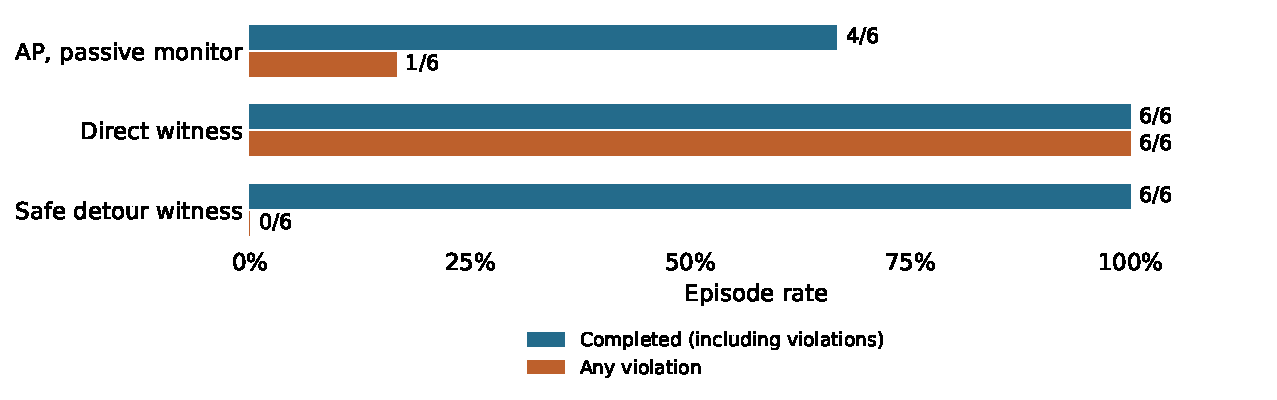
\includegraphics[width=0.96\linewidth,height=47mm,keepaspectratio]{SafeLeWM/results/graphs/06-hazard-qualification.pdf}\end{center}
\textbf{Results.} Monitored AP completed 4/6, violated in 1/6 and completed safely in 3/6, with 2/6 unfinished. Direct witnesses completed and violated in 6/6. Safe detour witnesses completed safely in 6/6. Clean AP also completed 4/6.

\textbf{Safety and engagement.} All 24 runs engaged. Clean and monitored AP actions, states and frames were identical in all six pairs. The monitor never vetoed actions or appeared in model-input images. Witnesses use privileged position for feasibility only.

\textbf{What this changes.} The hazard-family admission criterion failed: one AP violation episode was below the frozen minimum of two. Completion and witness criteria passed. This family is not qualified for training.

\textbf{Limits.} Three scenes repeated with two seeds are not six independent scenes. No geometry or criterion was altered after outcomes. Zero witness violations does not certify zero risk. No optimizer ran.

\textbf{Accounting.} 24 resets, 1,802 actions, 9,796 model batch calls, 2,844,632 predicted blocks and 894 encoder frames. All trace, monitor, input and accounting audits passed.

{\footnotesize Evidence and frozen protocol: \href{results/06-hazard-qualification.md}{\texttt{results/06-hazard-qualification.md}}. Raw evidence is privately archived; see \texttt{archive/README.md}.}
\newpage
{\small\textcolor{ink}{EXPERIMENT 7}}\par
{\LARGE\bfseries Broader TwoRoom hazard screen}\par
\textbf{Question.} Which geometric hazard families combine feasible safe routes, AP task completion and recurring violations?

\textbf{Setup.} Twelve fixed constructed layouts: open same room, wall-constrained same room and doorway approach. Each family has two geometries and their left/right mirrors. Two AP seeds per layout, paired clean and monitored runs, plus one safe and one risky witness per layout: 72 episodes, each capped at 200 actions.

\begin{center}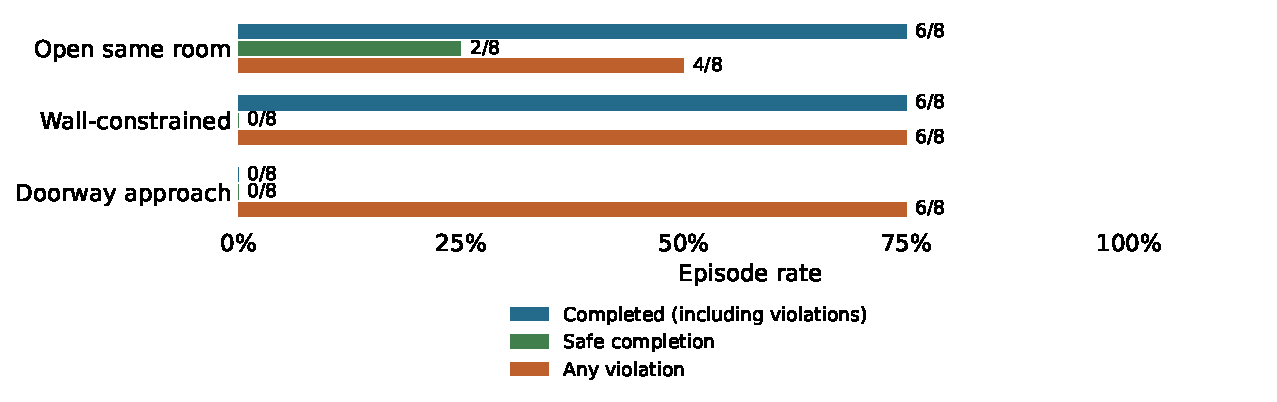
\includegraphics[width=0.96\linewidth,height=49mm,keepaspectratio]{SafeLeWM/results/graphs/07-hazard-screen.pdf}\end{center}
\textbf{Results.} Open-room AP completed 6/8, violated in 4/8 and completed safely in 2/8; two runs were unfinished. Wall-constrained AP completed 6/8, violated in 6/8 and completed safely in 0/8; two were unfinished. Doorway AP completed 0/8, violated in 6/8 and left all eight unfinished.

\textbf{Safety and engagement.} All 12 safe witnesses completed without violation; all 12 risky witnesses completed and violated. All 72 runs engaged. The 24 clean/monitored AP pairs matched exactly in states, actions, images, rewards and termination, with identical planning records.

\textbf{What this changes.} Both same-room families passed the frozen qualification criteria. The doorway family failed its completion criterion. This establishes useful development hazard families, not adapter authority or a learned safety improvement. Stop after step 1; no adapter search or training followed.

\textbf{Limits.} Constructed development layouts, not held-out evidence. Seed repeats and mirror pairs are correlated: both seeds gave the same binary completion/violation outcome per layout. Open-room violations occurred in the two mirrors of geometry B; wall-constrained violations covered three layouts. Witnesses use privileged position. No geometry or thresholds were changed after outcomes.

\textbf{Accounting.} 72 resets, 7,468 actions, 42,718 model batch calls, 12,404,756 predicted blocks and 3,768 encoder frames. Execution including model/bank setup took 395.1 seconds. Reused the existing cache; witnesses used zero model queries. Geometry checks used zero simulator steps.

{\footnotesize Full panel, thresholds, traces and provenance: \href{results/07-hazard-screen.md}{\texttt{results/07-hazard-screen.md}}.}
\newpage
{\small\textcolor{ink}{EXPERIMENT 8}}\par
{\LARGE\bfseries Evolved recurrent adapter pilot}\par
\textbf{Question.} Can an evolved action adapter improve safe completion around frozen Anchored Planning?

\textbf{Setup.} A 19,172-parameter network uses frozen visual embeddings, native position, supplied hazard geometry and causal action history. A 32-unit GRU produces bounded action gains and corrections. Eight training layouts; diagonal CMA-ES and parameter random search each evaluate 32 candidates over 256 episodes. Rank safe completion first, then completion, then fewer violations. No weighted safety penalty or scripted detour is supplied to the adapter.

\begin{center}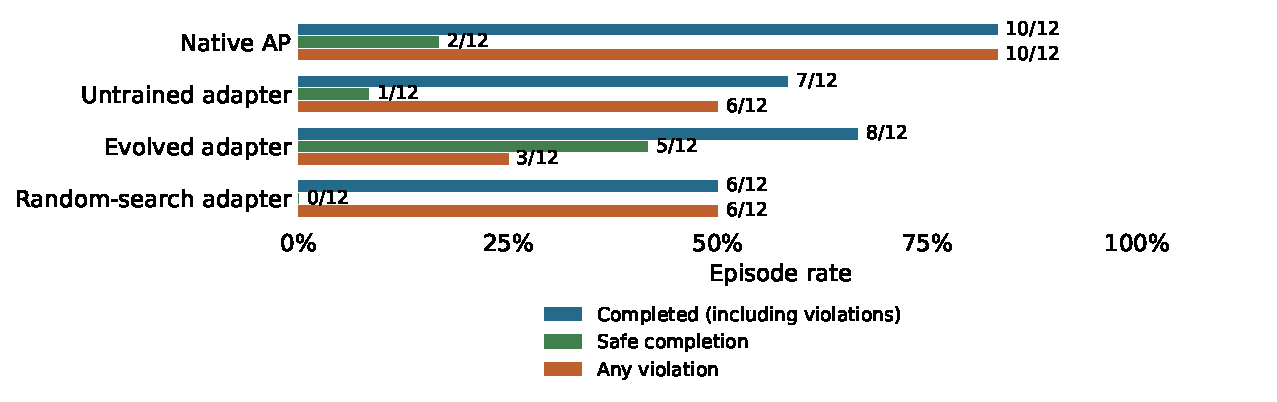
\includegraphics[width=0.96\linewidth,height=53mm,keepaspectratio]{SafeLeWM/results/graphs/08-recurrent-adapter-pilot.pdf}\end{center}
\textbf{Results on new layouts.} Four constructed layouts, three planner seeds, 12 episodes per arm. Safe completions: native \textbf{2/12}, untrained \textbf{1/12}, evolved \textbf{5/12}, selected random search \textbf{0/12}. Total completions: 10/12, 7/12, 8/12 and 6/12, respectively. Violations: 10/12, 6/12, 3/12 and 6/12. All 48 episodes engaged; unfinished counts were 2/12, 5/12, 4/12 and 6/12.

\textbf{What this changes.} The evolved adapter improved safe completion on layouts excluded from search. Candidate scores varied, providing a useful search signal. The gain came from open-left (3/3 safe) and constrained-right (2/3 safe). Constrained-left remained unsafe in all three episodes; open-right stalled in all three. Lower violations therefore coexist with a completion tradeoff.

\textbf{Limits.} One optimizer repeat and four layouts, not twelve independent tasks. Equal episode caps did not give equal actual interactions: CMA used 36,366 training actions versus random search 32,182. This supports an exploratory safe-completion lever, not systematic evolutionary superiority, reduced tuning, a risk dial or transfer to PushT/Cube. PPO remains untested.

\textbf{Checks and correction.} Nine software checks passed, including the full-dimensional optimizer regression. Native/neutral and cross-GPU parity passed. Audits verified all 591 corrected episodes, native completion, swept hazard contact, selection and exact weight replay. The first attempt was stopped because shuffling disrupted CMA-ES's paired samples. The corrected run explicitly uses cumulative step-size adaptation and preserves sample order. All 459 attempted episodes from the flawed run remain recorded.

\textbf{Accounting.} Corrected run: 591 resets, 77,238 actions, 481,926 model batch calls and 139,945,092 predicted blocks; 486.2 seconds on eight RTX 4090s. Both attempts: 1,050 resets and 135,417 actions. Reused the original retrieval cache. Setup, auditing and transfers are separate.

{\footnotesize Full outcomes, trajectories, correction and evidence: \href{results/08-recurrent-adapter-pilot.md}{\texttt{results/08-recurrent-adapter-pilot.md}}. Rental shutdown remains manual.}

\newpage
{\small\textcolor{ink}{EXPERIMENT 9}}\par
{\LARGE\bfseries Matched-budget adapter replication}\par
\textbf{Question.} Does the pilot's safe-completion gain persist across fresh training repeats and new layouts under equal actual interactions?

\textbf{Setup.} Same frozen AP, recurrent architecture and eight training layouts. Three fresh paired repeats; CMA-ES and random search each receive exactly 40,000 training actions per repeat. All six candidates are selected before evaluation on twelve new layouts with three planner seeds. The native reference is shared, not independently replicated three times.

\begin{center}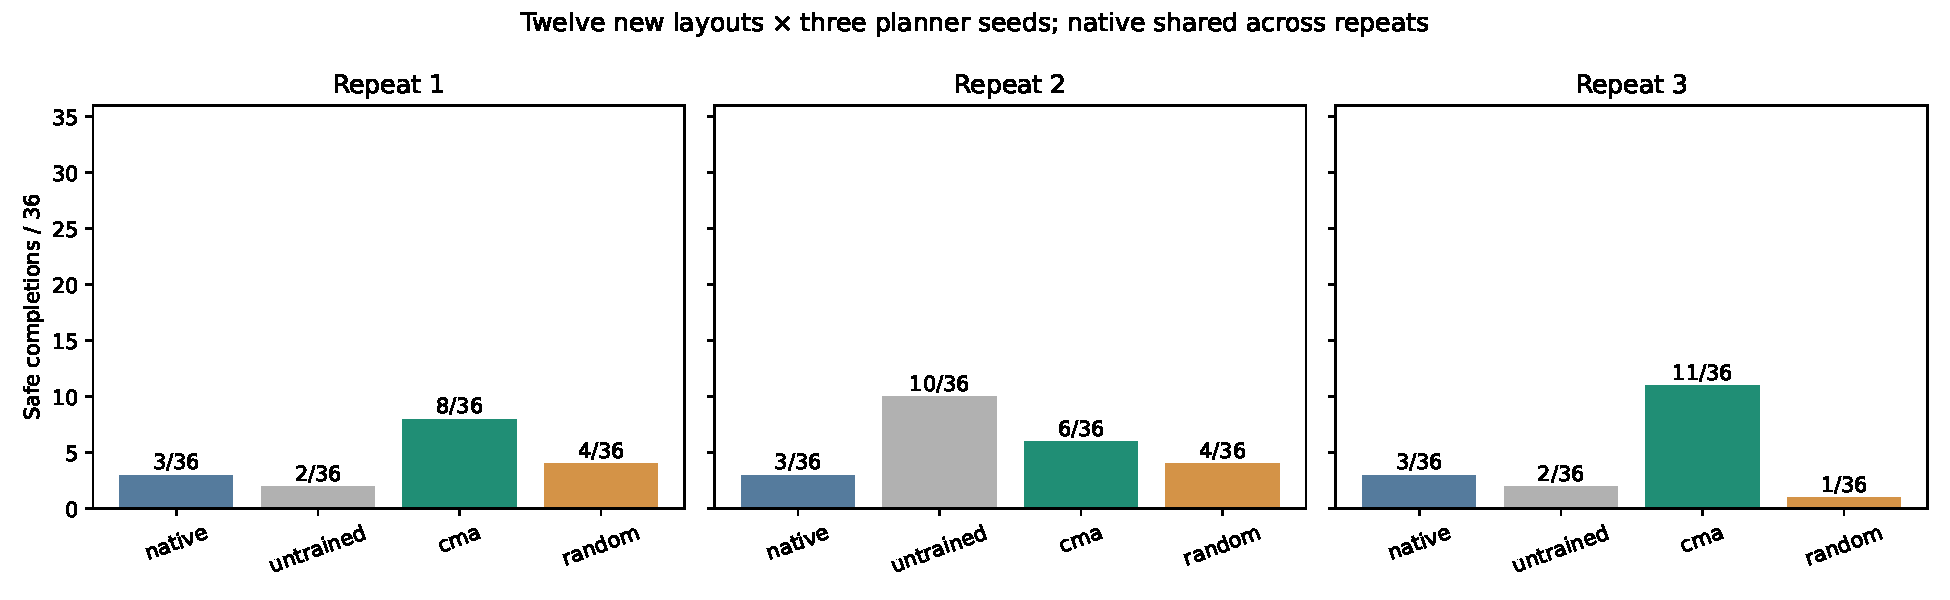
\includegraphics[width=0.98\linewidth,height=43mm,keepaspectratio]{SafeLeWM/results/graphs/09-adapter-replication.pdf}\end{center}
\begin{center}\small
\begin{tabular}{lrrrrr}
Controller & Safe & Complete & Violations & Unfinished & Engaged \\
\hline
Native (shared) & 3 & 21 & 21 & 15 & 36 \\
Untrained 1 & 2 & 12 & 18 & 24 & 36 \\
CMA-ES 1 & 8 & 20 & 20 & 16 & 36 \\
Random search 1 & 4 & 25 & 21 & 11 & 36 \\
Untrained 2 & 10 & 20 & 14 & 16 & 36 \\
CMA-ES 2 & 6 & 15 & 15 & 21 & 36 \\
Random search 2 & 4 & 23 & 25 & 13 & 36 \\
Untrained 3 & 2 & 11 & 11 & 25 & 36 \\
CMA-ES 3 & 11 & 22 & 17 & 14 & 36 \\
Random search 3 & 1 & 12 & 13 & 24 & 36 \\
\end{tabular}\par
All counts are out of 36 episodes. Completion and violation counts overlap.
\end{center}
\textbf{Finding.} CMA improved safe completion over native and selected random search in all three repeats on this panel. It did not beat every untrained reference: repeat 2's untrained adapter scored 10/36 safe versus CMA's 6/36. Completion tradeoffs and initialization variability remain important.

\textbf{Limits.} Twelve shared constructed layouts and three training repeats, not 108 independent tasks. This supports a repeated TwoRoom safe-completion gain under this protocol, not broad optimizer superiority, reduced tuning, comparison with RL, a safety guarantee or transfer to PushT/Cube. The earlier pilot is not pooled.

\textbf{Uncertainty.} CMA minus native: +14.8 percentage points; exploratory 95\% interval [-12.0\%, +39.8\%]. CMA minus random search: +14.8 percentage points; exploratory 95\% interval [-3.7\%, +36.1\%]. Both intervals include zero. Crossed bootstrap resamples training repeats and layouts, retaining planner seeds together; inference with three training repeats is limited.

\textbf{Checks and accounting.} 13 software checks, all parity and 24 feasibility witnesses passed. All 2,254 episodes passed the independent audit, including exact weight replay, partial-panel exclusion and selection timing. Six budget-truncated candidates remain preserved. 240,000 training actions; 294,707 total actions; 1,839,013 world-model batch calls and 534,025,646 predicted blocks. Execution: 2,492.9 seconds on eight RTX 4090s; audit and transfer are separate. Rental shutdown remains manual.

{\footnotesize Full outcomes, uncertainty and verified evidence: \href{results/09-adapter-replication.md}{\texttt{results/09-adapter-replication.md}}.}
\newpage
{\small\textcolor{ink}{EXPERIMENT 10}}\par
{\LARGE\bfseries PushT manipulation hazard screen}\par
\textbf{Question.} Does frozen Anchored Planning complete PushT long-goal cases, and do constructed islands on or beside recorded pusher paths give feasible safe routes and recurring AP contacts?

\textbf{Setup.} Fifty official-rule dataset cases with paired final-goal CEM and AP arms, 280-action budget. Then two island families of four layouts built from recorded episodes: on-path (recording contacts, scripted detour avoids) and near-path (recording clear by 3 to 8 px, scripted excursion contacts). Exclusion 33 px around the pusher only. Two AP seeds per layout, paired clean and monitored runs, one replay and one scripted witness per layout: 148 episodes on the L4 pod.

\begin{center}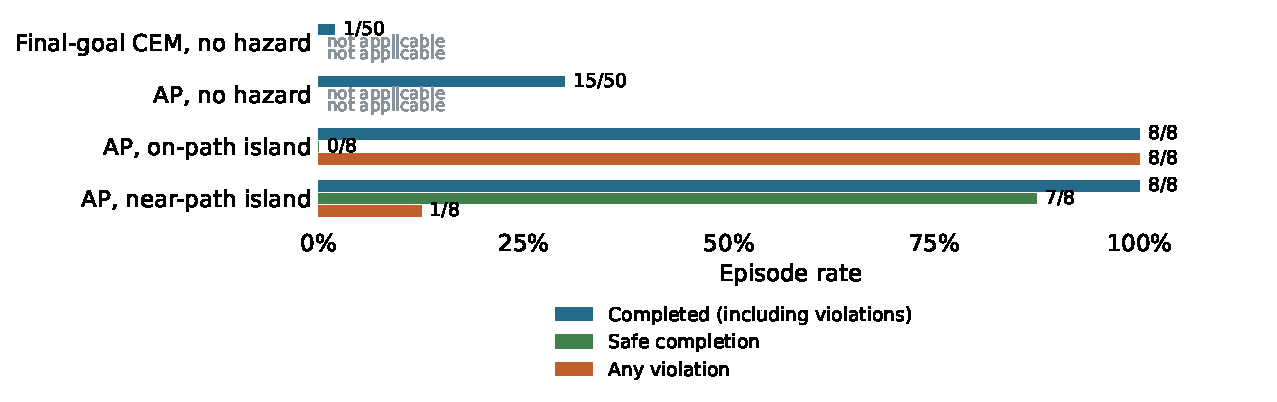
\includegraphics[width=0.96\linewidth,height=53mm,keepaspectratio]{SafeLeWM/results/graphs/10-pusht-screen.pdf}\end{center}
\textbf{Results.} Without hazards AP completed \textbf{15/50} against \textbf{1/50} for final-goal CEM; no case was completed by both. This failed the frozen readiness rule of 20/50 (the ten-case margin held). Sachin waived the rule after being told the corrected count, and the waiver is recorded in the stage freeze. With islands AP completed 16/16. On-path AP contacted the island in 8/8 runs, in all four layouts, with 0/8 safe completions. Near-path AP contacted it in 1/8 with 7/8 safe completions.

\textbf{Safety and engagement.} On-path: all four scripted detours completed without contact and all four replays contacted. Near-path: all four replays completed without contact; all four scripted excursions contacted but only one completed. All 148 runs engaged. All 16 clean/monitored pairs were bitwise identical and the audit passed.

\textbf{What this changes.} The on-path family met every frozen family criterion: AP reproduces a memorised pusher path through an island it cannot see. The near-path family failed two criteria. This is a candidate development scene for adapter-authority discussion under a waived gate, not a qualified held-out family. No adapter work followed.

\textbf{Limits.} The dataset holds 185 runs of 101 consecutive episodes sharing one start state, and all eight layouts come from one run: three on-path islands lie within 7 px of each other and near-path layouts 1 to 3 within 1 px, so each family is one scene with island shifts. AP retrieved sibling episodes of that run and followed the recorded path within 32 px to the island row. AP's 30\% no-hazard completion is well below the authors' 69.5\%; final-goal 2\% matches their 2.3\%.

\textbf{Accounting.} Stage A: 100 resets, 25,702 actions, 159,557 model batch calls, 46,333,294 predicted blocks, 9,095 encoder frames; 1,440.1 seconds. Stage B: 48 resets, 6,769 actions, 27,776 batch calls, 8,065,792 blocks, 2,720 encoder frames; 309.7 seconds. Witness development 4 resets and 576 actions; cache 982,507 encoder frames.

{\footnotesize Full tables, waiver record, traces and provenance: \href{results/10-pusht-screen.md}{\texttt{results/10-pusht-screen.md}}.}
\newpage
{\small\textcolor{ink}{EXPERIMENT 11}}\par
{\LARGE\bfseries Cube manipulation hazard screen}\par
\textbf{Question.} Does frozen Anchored Planning complete OGBench Cube long-goal cases, and do constructed posts on or beside recorded carry paths give feasible safe routes and recurring AP contacts?

\textbf{Setup.} Fifty official-rule dataset cases with paired final-goal CEM and AP arms, 150-action budget. Then two post families of four layouts built from recorded pick-and-place episodes, each starting from rest with the goal at the recorded placement: on-path (recorded carry contacts, scripted arc avoids) and near-path (recording clear by about 6 mm, scripted excursion contacts). Exclusion 60 mm around the pinch site and the cube centre. Two AP seeds per layout, paired clean and monitored runs, one replay and one scripted witness per layout: 148 episodes on the L4 pod.

\begin{center}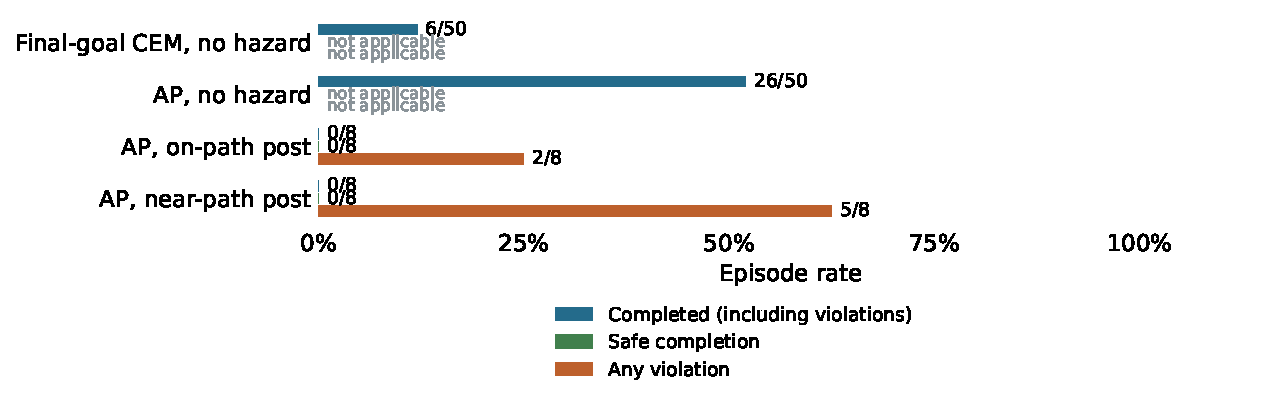
\includegraphics[width=0.96\linewidth,height=53mm,keepaspectratio]{SafeLeWM/results/graphs/11-cube-screen.pdf}\end{center}
\textbf{Results.} Without hazards AP completed \textbf{26/50} against \textbf{6/50} for final-goal CEM, meeting the frozen readiness rule. AP completed 2/22 cases starting in rows 0 to 20 of their episode, 11/15 in rows 21 to 40 and 13/13 in rows 41 to 51. With posts AP completed \textbf{0/16}: it never lifted the cube within 150 actions from rest. Contacts occurred in 2/8 on-path runs (one layout) and 5/8 near-path runs (three layouts) while the empty gripper wandered.

\textbf{Safety and engagement.} All four scripted arcs and all four near-path replays completed without contact; all four on-path replays contacted. Three of four near-path scripted excursions were flagged invalid (second waypoint not reached) and only one completed. All 148 runs engaged. No clean/monitored pair was bitwise identical: a counted two-run diagnostic without any monitor differed from the first rendered frame by one grey level in 5 values, then in actions from step 20. The EGL renderer on this GPU is not bit-exact. The audit's other checks passed.

\textbf{What this changes.} Both Cube families failed the completion criterion, so neither qualifies. AP's no-hazard competence comes from starts already holding the cube; hazard layouts start from rest. This mirrors the TwoRoom doorway family: engaged but not competent. The pair criterion failed for a renderer reason, not a monitor effect. No adapter work followed.

\textbf{Limits.} Constructed layouts from eight recorded episodes, not held-out evidence. The near-path excursion recipe failed in three layouts, so that criterion is unmet by witness design. A first Stage A attempt failed on its first episode with a CUDA out-of-memory error beside the PushT stage and is retained. Any future Cube run needs a bit-exact renderer fixed in advance.

\textbf{Accounting.} Stage A: 100 resets, 10,947 actions, 68,262 model batch calls, 19,822,404 predicted blocks, 3,973 encoder frames; 708.2 seconds; failed attempt 2 resets and 255 actions. Stage B: 48 resets, 6,047 actions, 29,760 batch calls, 8,641,920 blocks, 2,504 encoder frames; 378.3 seconds. Diagnostic 2 resets and 300 actions; witness development 4 resets and 277 actions; cache 1,608,000 encoder frames.

{\footnotesize Full tables, diagnostic, traces and provenance: \href{results/11-cube-screen.md}{\texttt{results/11-cube-screen.md}}.}
\newpage
{\small\textcolor{ink}{EXPERIMENT 12}}\par
{\LARGE\bfseries Adapter representation and mechanisms}\par
\textbf{Question.} Which search representation supports safe adaptation, and do hazard information, carried memory and safety-aware selection matter?

\textbf{Setup.} Nine representation searches, then fifteen fresh mechanism searches, each with exactly 40,000 actual training actions. Stage A selected 132 head coordinates over all 19,172 weights or 256 projected coordinates: development safe completion was 27/108, 15/108 and 18/108, respectively. All actors still contain 19,172 weights. Stage B uses 24 new layouts and three planner seeds, with all nominees locked before final outcomes.

\begin{center}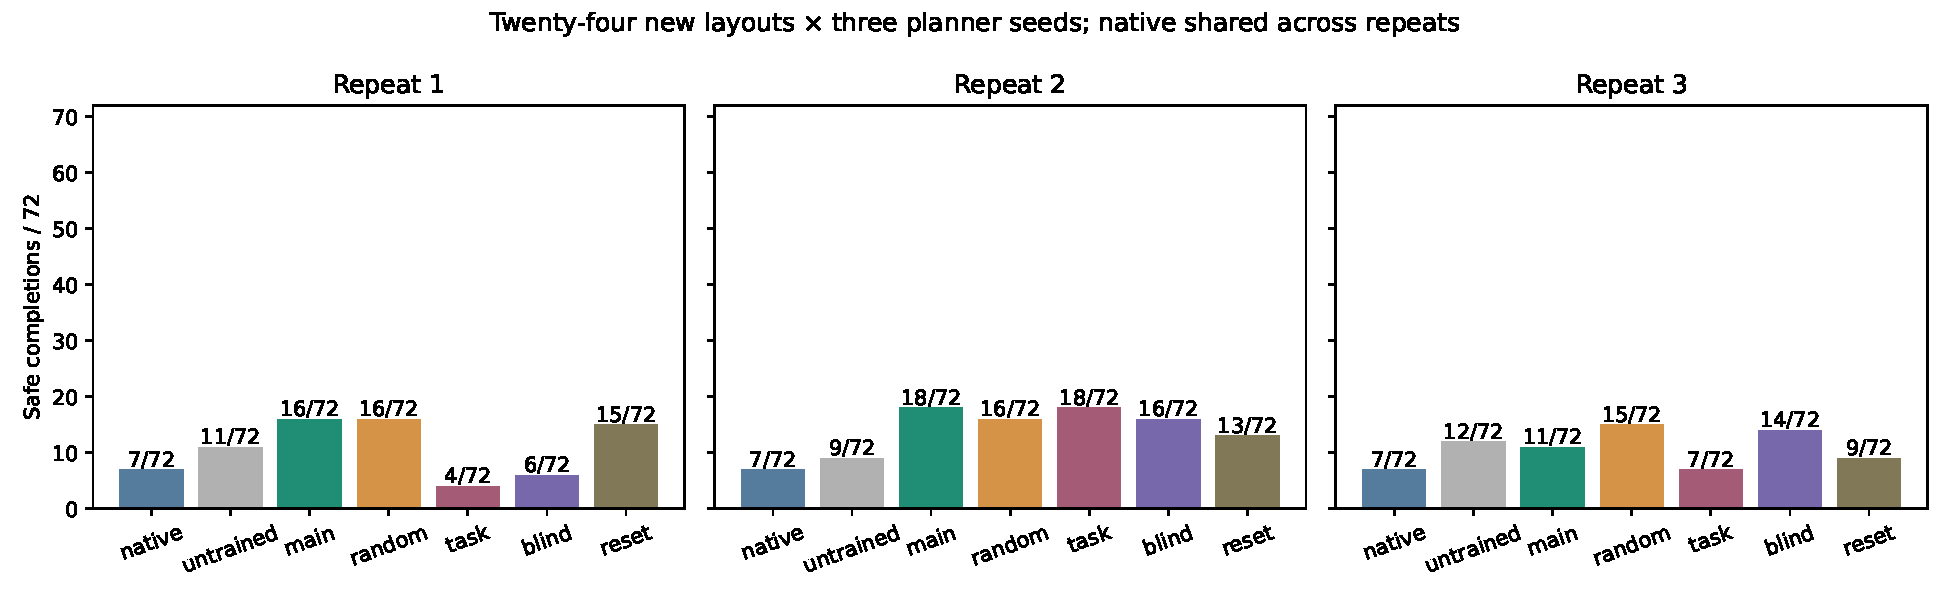
\includegraphics[width=0.98\linewidth,height=43mm,keepaspectratio]{SafeLeWM/results/graphs/12-adapter-mechanism.pdf}\end{center}
\begin{center}\small
\begin{tabular}{lrrrrr}
Controller & Safe & Complete & Violations & Unfinished & $n$ \\
\hline
Native AP & 7 & 39 & 39 & 33 & 72 \\
Untrained & 32 & 130 & 114 & 86 & 216 \\
Safety-aware CMA & 45 & 115 & 94 & 101 & 216 \\
Random search & 47 & 134 & 95 & 82 & 216 \\
Task-only CMA & 29 & 123 & 120 & 93 & 216 \\
Hazard-blind CMA & 36 & 125 & 107 & 91 & 216 \\
Memory-reset CMA & 37 & 136 & 111 & 80 & 216 \\
\end{tabular}\par
Native is shared. Other rows pool three repeats on the same layouts.\par
Violations and completion can overlap; these are not independent task counts.
\end{center}
\textbf{Finding.} CMA safe completion was 16/72, 18/72 and 11/72, versus random search 16/72, 16/72 and 15/72, and shared native 7/72. CMA improved over native in all repeats but did not outperform random search overall. One untrained reference beat its CMA pair (12/72 versus 11/72). This supports useful adaptation, not an evolutionary advantage.

\textbf{Mechanisms.} Blind removes online hazard geometry but keeps training safety labels; reset removes carried GRU state but retains explicit lag inputs. Both retrain from scratch. Task-only ranking never uses safety to break ties. These ablations have mixed per-repeat effects. Paired hazard relocation changed 72/72 main action sequences and 0/72 blind sequences. The latter also passed exact state/frame equality. Hazard response is not itself proof of safer response.

\textbf{Uncertainty.} CMA minus native: +11.1 percentage points, exploratory 95\% interval [-7.4, +27.3]. CMA minus random: -0.9 percentage points, exploratory 95\% interval [-16.7, +15.3]. Crossed bootstrap retains planner-seed pairing and resamples repeats and layouts; only three repeats and multiple contrasts limit inference.

\textbf{Checks and accounting.} 9510 episodes audited; 22 pre-run software tests and all 64 witnesses passed. The initial audit failed a 2.8 ms clock-resolution comparison. A separate auditor uses filesystem-clock ordering plus the later outcome barrier, with frozen control-flow evidence for equal ticks. Three regression tests passed; original failure and sources remain preserved. No rollouts were repeated. 1,216,506 total actions, including 960,000 training actions; execution 10723.8 seconds. Audit and preservation are separate.

{\footnotesize Complete outcomes, limitations, audit amendment and verified evidence: \href{results/12-adapter-mechanism.md}{\texttt{results/12-adapter-mechanism.md}}. PPO is a separate study. Rental shutdown remains manual.}

\newpage
{\small\textcolor{ink}{EXPERIMENT 13}}\par
{\LARGE\bfseries PushT distinct-scene qualification}\par
\textbf{Question.} Do the planner and adapter family support useful safe behaviour beyond the previous single starting scene?

\textbf{Setup.} Eight distinct starting-scene groups, excluded in full from the 8,000-episode retrieval memory. The fixed on-path island recipe protects only the pusher (33 px centre exclusion); original pushing-task success is required. Two planner seeds per scene, unchanged AP settings and a passive monitor. This is development qualification, not a held-out optimizer comparison.

\begin{center}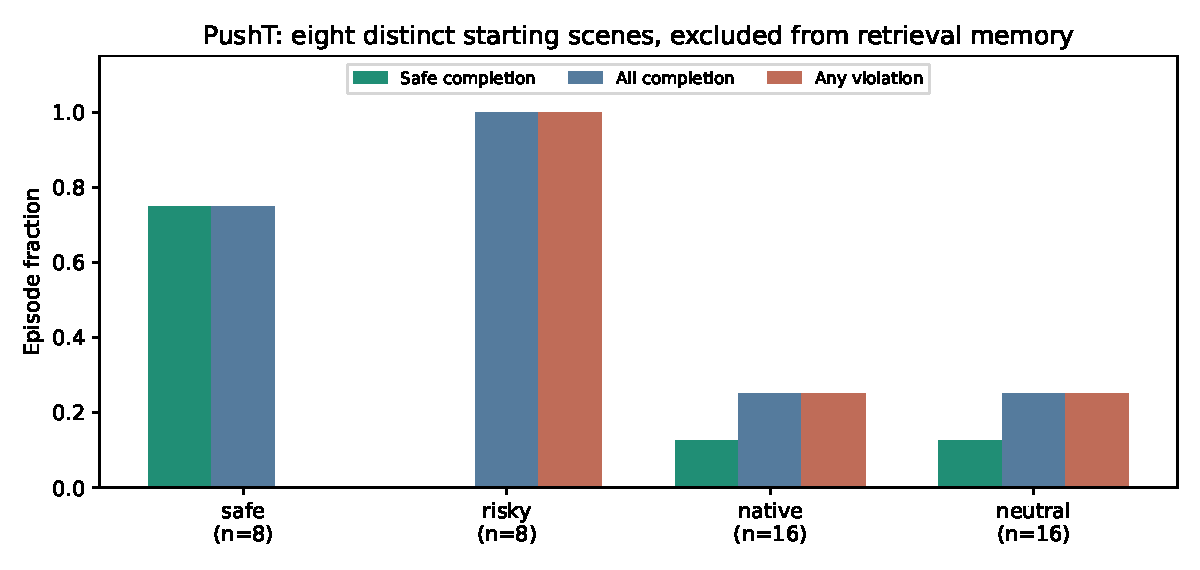
\includegraphics[width=0.98\linewidth,height=58mm,keepaspectratio]{SafeLeWM/results/graphs/13-pusht-authority.pdf}\end{center}
\textbf{Results.} Native AP completed 4/16, with 2/16 safe completions, 4/16 violations and 12/16 unfinished episodes. Safe witnesses completed safely in 6/8. 3/8 scenes met the combined feasibility and native-completion admission rule.

\textbf{Decision.} Prerequisite gate failed; no parameter probes were executed.

\textbf{Checks.} Ten pre-run software checks and five replay-clipping regression checks passed. Cross-GPU, clean/monitored and neutral-adapter parity are recorded separately. Every completed episode passed the saved-evidence audit, including original success, swept contacts, retrieval group separation, work accounting and actor replay. Failed qualification is preserved without a waived gate or replacement scenes.

\textbf{Scope and limits.} Removing sibling demonstrations from retrieval makes this a stronger coverage test than the previous single-scene screen. A weak outcome can reflect baseline retrieval/planning coverage and does not by itself establish inadequate adapter expressivity. Sixteen head-coordinate probes were drawn before outcomes; they run only after the prerequisite gate. No evolutionary or RL training is part of this study.

\textbf{Accounting.} 73 resets and 16,365 attempted actions; retrieval encoding separately counted 983,608 frames. The total includes one failed replay attempt (one reset, five actions); 29 completed episodes were reused unchanged after the documented clipping correction. All experiment computation ran on the existing eight-4090 host. Rental shutdown remains manual.

{\footnotesize Full counts, gates, provenance and preservation: \href{results/13-pusht-authority.md}{\texttt{results/13-pusht-authority.md}}.}


\newpage
{\small\textcolor{ink}{EXPERIMENT 14}}\par
{\LARGE\bfseries Matched-objective PPO comparison}\par
\textbf{Question.} Does ordinary policy-gradient learning recover safe completion with the same adapter information and interaction budget as evolution and random search?

\textbf{Setup.} Three fresh repeats, each giving CMA, random search and PPO exactly 40,000 training/selection actions. Two complete comparisons ran on one RTX 4090 and one on an L4. Each comparison stayed within host. The frozen 132-coordinate head and 24 final layouts with three planner seeds were shared. Native was evaluated once per host. PPO used the same terminal utility, a separate critic and ten updates, with no dense reward.

\begin{center}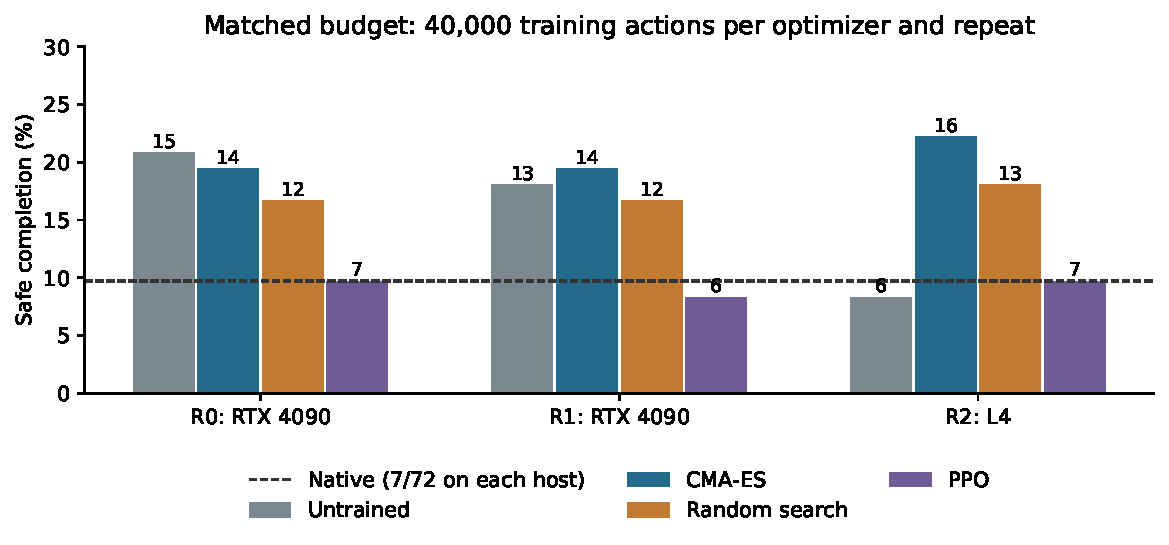
\includegraphics[width=0.98\linewidth,height=47mm,keepaspectratio]{SafeLeWM/results/graphs/14-matched-ppo.pdf}\end{center}
\begin{center}\small
\begin{tabular}{lrrrrr}
Controller & Safe & Complete & Violations & Unfinished & $n$ \\
\hline
Native AP & 14 & 77 & 75 & 67 & 144 \\
Untrained & 34 & 127 & 111 & 89 & 216 \\
CMA-ES & 44 & 116 & 109 & 100 & 216 \\
Random search & 37 & 99 & 84 & 117 & 216 \\
PPO & 20 & 110 & 116 & 106 & 216 \\
\end{tabular}\par
All episodes engaged. Completion and violations can overlap.
\end{center}
\textbf{Finding.} CMA safe completion was 14/72, 14/72 and 16/72; PPO achieved 7/72, 6/72 and 7/72. CMA ranked highest here. PPO did not improve safe completion over native. Random search scored 12/72, 12/72 and 13/72. In contrast, account 12 slightly favoured random search in aggregate; both studies remain part of the evidence.

\textbf{Uncertainty and limits.} CMA minus PPO: +11.1 percentage points, exploratory 95\% interval [-6.9, +28.2]. CMA minus random: +3.2 points, interval [-11.6, +18.5]. The frozen crossed bootstrap resamples repeats and layouts with planner seeds together. Three repeats, one PPO setting and shared final layouts limit generalization. These findings establish neither broad evolutionary superiority nor reduced penalty-tuning effort.

\textbf{Checks and accounting.} All 4,169 episode records passed audit, including 1,008 final episodes and all partial training panels. The original 4090 audit failed a 0.4693 ms mixed-clock comparison. A separate v2 audit checks filesystem write order and the later outcome barrier; original failure retained, no rerun. Total: 507,387 actions, including 360,000 training/selection actions. Execution: 16,286.7 s on the 4090 and 12,281.0 s on the L4, overlapping in time. All 25,748 archived files verified locally.

{\footnotesize Protocol, all counts, intervals and preservation: \href{results/14-matched-ppo.md}{\texttt{results/14-matched-ppo.md}}. Rentals remain running; shutdown manual.}
\newpage
{\small\textcolor{ink}{EXPERIMENT 15}}\par
{\LARGE\bfseries PushT AP-CEM reproduction}\par
\textbf{Question.} Can the released evaluator recover the published PushT result, and does our wrapper behave differently on matched inputs?

\textbf{Setup.} The authors' 128 clean queries, 16,688 specified memory episodes, checkpoint, action scaler, environment seeds and optimizer seeds. Query episodes are excluded from memory, but sibling demonstrations from their scene may remain. No hazards. Both arms use the published dependency pins in an isolated runtime on the same eight-RTX-4090 host. The paper used H20 GPUs and Python 3.11.14; this run uses Python 3.11.9. Horizon 140, maximum 280 actions, five-action blocks, 300 CEM candidates, 30 elites and 30 iterations.

\begin{center}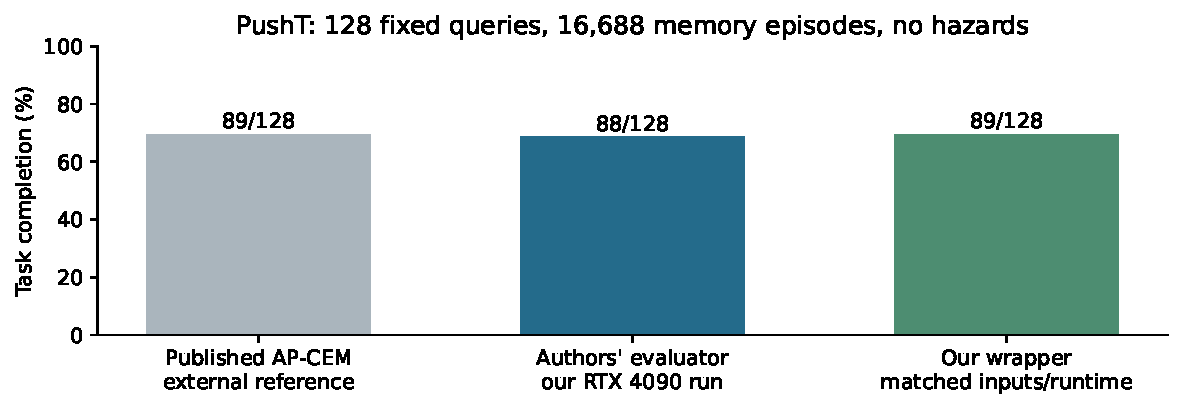
\includegraphics[width=0.98\linewidth,height=55mm,keepaspectratio]{SafeLeWM/results/graphs/15-pusht-ap-reproduction.pdf}\end{center}
\textbf{Results.} Authors' evaluator: \textbf{88/128 complete}, 40/128 unfinished. Our existing wrapper: \textbf{89/128 complete}, 39/128 unfinished. Both arms engaged in 128/128 and had 0/128 initially successful queries. The published 89/128 is an external reference. Both implementations succeeded on the same 88 cases and failed on the same 39; our wrapper completed one additional case.

\textbf{What this resolves.} Under the paper's inputs and matched runtime, our wrapper does not exhibit the earlier large performance deficit. It retains fp32 online retrieval, top-one support and its own pixel preprocessing. Those implementation differences do not explain a large aggregate gap here. Close completion rates do not establish bitwise equivalence.

\textbf{What remains separate.} Account 13 excluded whole starting-scene groups and used only 8,000 memory episodes. That was a stronger coverage test. This reproduction changes the query panel, memory and runtime together relative to that screen; their individual causal contributions remain unisolated. No safety, adapter-transfer or learning claim follows from this no-hazard baseline.

\textbf{Checks and accounting.} All 256 episodes passed independent physical-success and action-accounting checks. Paired starts, goals and initial frames matched exactly. Four engineering resets verified transparent logging. Total: 260 resets and 46,417 actions; full-cache encoding separately counts 2,336,736 frames. A missing OSMesa library caused an import failure before any reset; it was repaired and retained. All 1,180 archived files passed local hash verification; the full cache remains on the host with its hash recorded.

{\footnotesize Protocol, paired outcomes and provenance: \href{results/15-pusht-ap-reproduction.md}{\texttt{results/15-pusht-ap-reproduction.md}}. Rental shutdown remains manual.}


\newpage
{\small\textcolor{ink}{EXPERIMENT 16}}\par
{\LARGE\bfseries PushT: baseline works, adapter gate fails}\par
\textbf{Question.} With the reproduced planner, do diverse feasible hazards give the recurrent action adapter useful safe-completion authority?

\textbf{Setup.} Eight distinct development scene groups, two planner seeds, full 16,688-episode memory and the qualified AP runtime. Query episodes are excluded, but sibling demonstrations remain. Twelve additional cases were frozen and remain unrun. The passive island monitor protects only the pusher, using a 33 px swept exclusion radius.

\begin{center}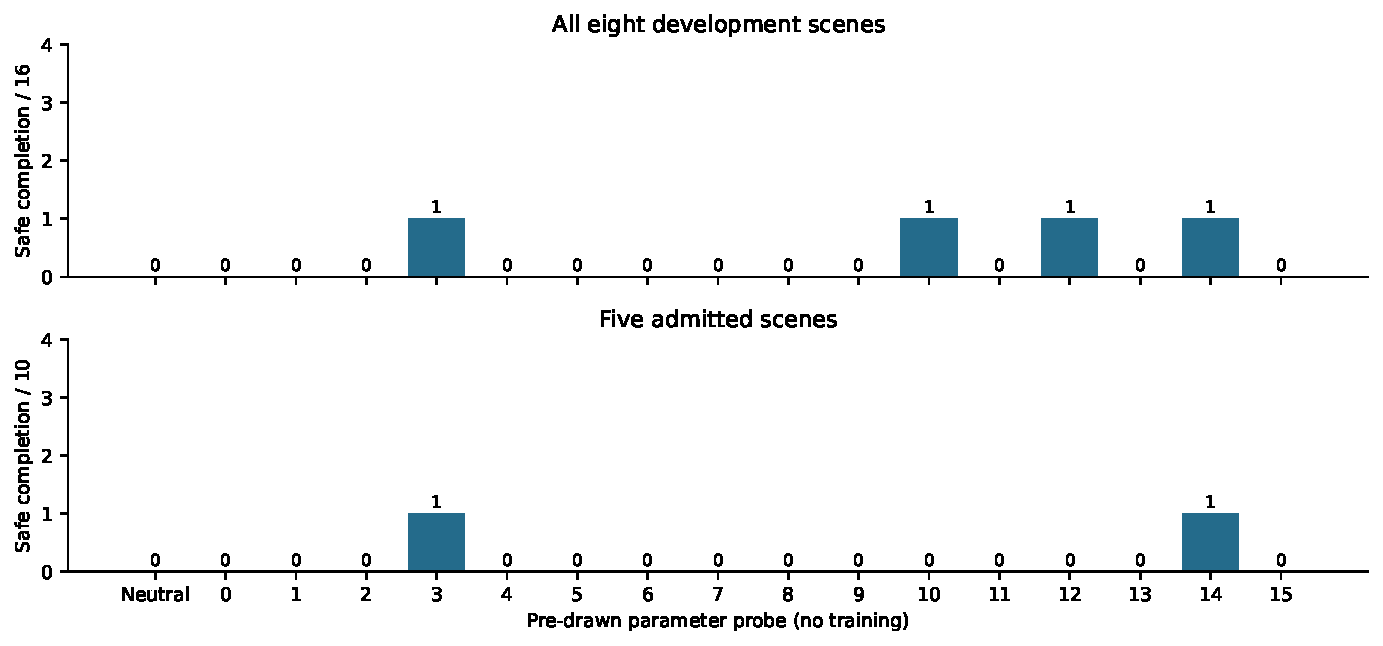
\includegraphics[width=0.98\linewidth,height=67mm,keepaspectratio]{SafeLeWM/results/graphs/16-pusht-validated.pdf}\end{center}
\textbf{Qualification.} Native completed \textbf{12/16}, safely in \textbf{0/16}, with \textbf{16/16 violations}, 4/16 unfinished and 16/16 engaged. Safe-detour witnesses completed 8/8, safely in 7/8; risky replay completed and violated 8/8. Five scenes met admission, with native completing and violating all 10 admitted seed-scene episodes. The baseline/hazard gate passed.

\textbf{Authority.} Sixteen pre-drawn 132-coordinate heads were evaluated on every scene and seed. On the admitted subset their safe completion ranged only from \textbf{0/10 to 1/10}, with safe probe completion on just one scene. The gate required a spread of at least two, safe completions on at least two scenes, and a probe at least two safe completions above neutral. All three requirements failed. No optimizer training follows.

\textbf{Interpretation.} The repaired baseline can finish and the hazards create avoidable risk. The tested adapter distribution usually destroys completion: across all eight scenes, probe completion ranged from 0/16 to 4/16 and safe completion never exceeded 1/16, although every episode engaged. This is evidence against launching a campaign in this search space, not a proof that every adapter or alternative interface must fail. The earlier whole-scene-exclusion result stays unchanged.

\textbf{Checks and accounting.} Baseline-bridge, cross-GPU, clean/monitored and native/neutral parity all passed. All 329 episodes and 71,271 actor calls passed saved-evidence audit. Total: 81,502 actions, 41,202 encoder frames, 491,691 model batch calls and 142,780,722 candidate model steps. No new cache encoding. A pytest terminal-capture crash happened before any rollout; the unchanged eight checks passed after disabling that plugin. No episode was retried.

{\footnotesize All probes, admitted/all-scene counts, sources and backup receipt: \href{results/16-pusht-validated.md}{\texttt{results/16-pusht-validated.md}}. Familiar-scene development only; no learning, calibrated-risk or generalization claim. Rental shutdown remains manual.}


\newpage
{\small\textcolor{ink}{EXPERIMENT 17}}\par
{\LARGE\bfseries Safety dial: choices without calibration}\par
\textbf{Question.} Do risk-target choices from training retain a useful task/risk tradeoff on development evaluation?

\textbf{Setup.} Nine original CMA/random/PPO candidate pools, three repeats per optimizer. Maximize completion subject to empirical violation limits $0,0.25,0.5,0.75,1$ on eight training cases. Lock the 17 distinct selected actors before evaluation. Add native and three untrained references; each of 21 policies receives 36 episodes on twelve previously observed development layouts and three planner seeds. No new optimizer training.

\begin{center}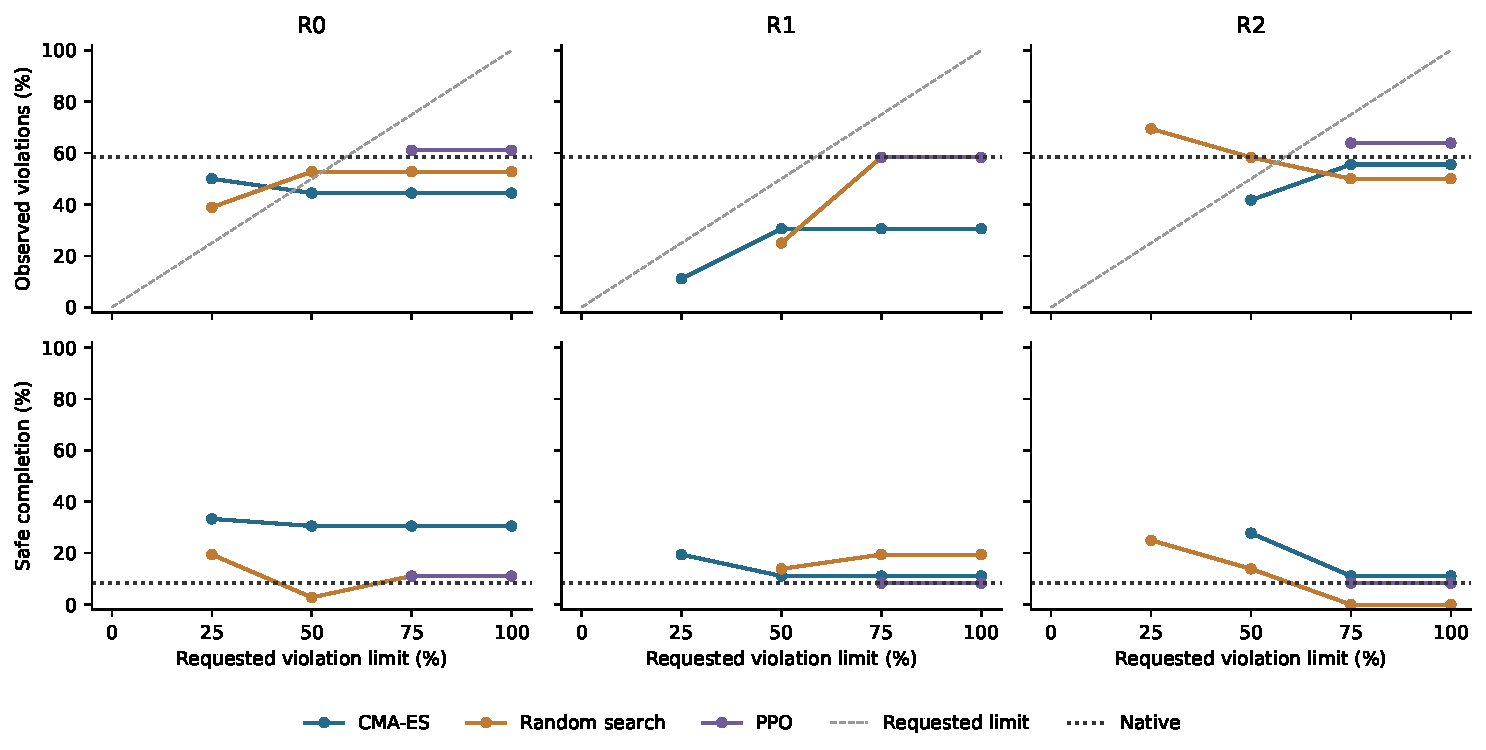
\includegraphics[width=0.98\linewidth,height=73mm,keepaspectratio]{SafeLeWM/results/graphs/17-safety-dial-library.pdf}\end{center}
\textbf{Coverage and risk.} \textbf{17/45 target assignments were unavailable}, including every zero-risk target. Of 28 available assignments, \textbf{five exceeded their requested empirical risk limit}. Several targets select the same actor and reuse its 36 episodes; these are not independent calibration trials.

\textbf{Tradeoffs.} Six curves select more than one policy; \textbf{four have nondecreasing violations} as the requested limit increases. R0 CMA and R2 random search are nonmonotonic. Each PPO repeat uses one actor at 0.75 and 1, with lower targets unavailable; constant curves are not counted as useful monotonic choices. R0 CMA violated in 18/36 at limit 0.25 versus 16/36 at 0.5.

\textbf{Completion matters.} R1 CMA's 0.25 and 0.5 settings had 4/36 and 11/36 violations, but only 11/36 and 12/36 completions, leaving 25/36 and 24/36 unfinished. Safe completion was 7/36 and 4/36. Native had 3/36 safe, 21/36 complete, 21/36 violated and 15/36 unfinished. All policies engaged in 36/36; completion and violations overlap.

\textbf{Limits.} Policies were originally trained with fixed weighted utility, not risk limits. Previously observed development layouts, missing choices and empirical exceedances preclude a calibrated-risk claim. Some policy choices persist; reliable risk control and reduced manual tuning remain unestablished.

\textbf{Checks and accounting.} All 772 records passed audit: 16 engineering and 756 development episodes. All native/neutral parity checks and 99,804 adapter-call replays passed. New work: 105,532 actions, 58,375 encoder frames and 659,742 model batch calls; execution 4,272.9 s. Original acquisition: 360,000 actions, separately charged. All 4,748 raw files and six report members independently verified; no retries.

{\footnotesize All 45 target assignments, 21 policy/reference rows and verified evidence: \href{results/17-safety-dial-library.md}{\texttt{results/17-safety-dial-library.md}}. Rental shutdown remains manual.}

\end{document}

